\chapter{Meilensteinplanung}
Im Rahmen dieses Projekts wurde eine umfassende Planung und Organisation der Arbeitspakete durchgeführt. 
Dies umfasste die Analyse der Tabelle mit den Arbeitspaketen sowie die Erstellung eines Gantt-Diagramms. 
Letzteres bietet eine visuelle Darstellung der zeitlichen Abfolge und Dauer der verschiedenen Aufgaben, was die Projektplanung und -kontrolle erleichtert.

\section{Vorgehensweise zur Erstellung des Gantt-Diagramms}
Zunächst wurden alle relevanten Daten aus den Arbeitspaketen extrahiert und aufbereitet.
Die Tabelle enthält die zwei wesentlichen Spalten \enquote{Beschreibung} und \enquote{Dauer}.
Zur Erstellung des Gantt-Diagramms wurde die Website \texttt{onlinegantt.com} in Anspruch genommen.
Diese Plattform bietet eine benutzerfreundliche Oberfläche zur Eingabe und Visualisierung von Projektplänen.\newline
Für jedes Arbeitspaket wurde das Startdatum gemäß der Tabelle eingetragen.
Dabei wurde die Aufgabenbeschreibung als Titel für die jeweiligen Arbeitspakete zusammengefasst.
Die Dauer der Aufgaben wurde entsprechend der Tabelle kategorisiert und entweder in Tagen oder Wochen angegeben.\newline
Dadurch wird die zeitliche Abfolge der Aufgaben visualisiert, um mögliche Überschneidungen oder Abhängigkeiten zu erkennen. 
Die Erstellung des Gantt-Diagramms zeigt die klare Struktur des Projekts im Zeitraum von 08.03.2024 bis 18.06.2024. 
Die logische und sequenzielle Anordnung der Aufgaben erleichtert die Nachverfolgung und Kontrolle des Projekts.

\section{Planung der Arbeitspakete}
Dabei beanspruchen einige Aufgaben, wie in etwa die Einrichtung des GitHub-Repositories oder die Erstellung der Projektstruktur, nur einen Tag. 
Andere Aufgaben, wie die Implementierung des Chat-Screens oder die Anpassung der Seiten-Navigation, erstrecken sich über mehrere Wochen aufgrund der Komplexität und der Zeit für das Lösen von auftretenden Fehlern beim Testen.
Diese kürzeren Aufgaben wurden in verschiedenen Sprints parallel zu den umfangreicheren Aufgaben geplant, um die Gesamtdauer des Projekts zu minimieren und schneller Fortschritte sehen zu können.

\section{Visualisierung}
Durch das Gantt-Diagramm konnten potenzielle Engpässe und Risiken identifiziert werden.
Ein besonderes Augenmerk gilt Aufgaben, die kritische Pfade darstellen, um Verzögerungen zu vermeiden.

\begin{figure}[H]
    \caption[Meilensteinplanung]{Meilensteinplanung}
    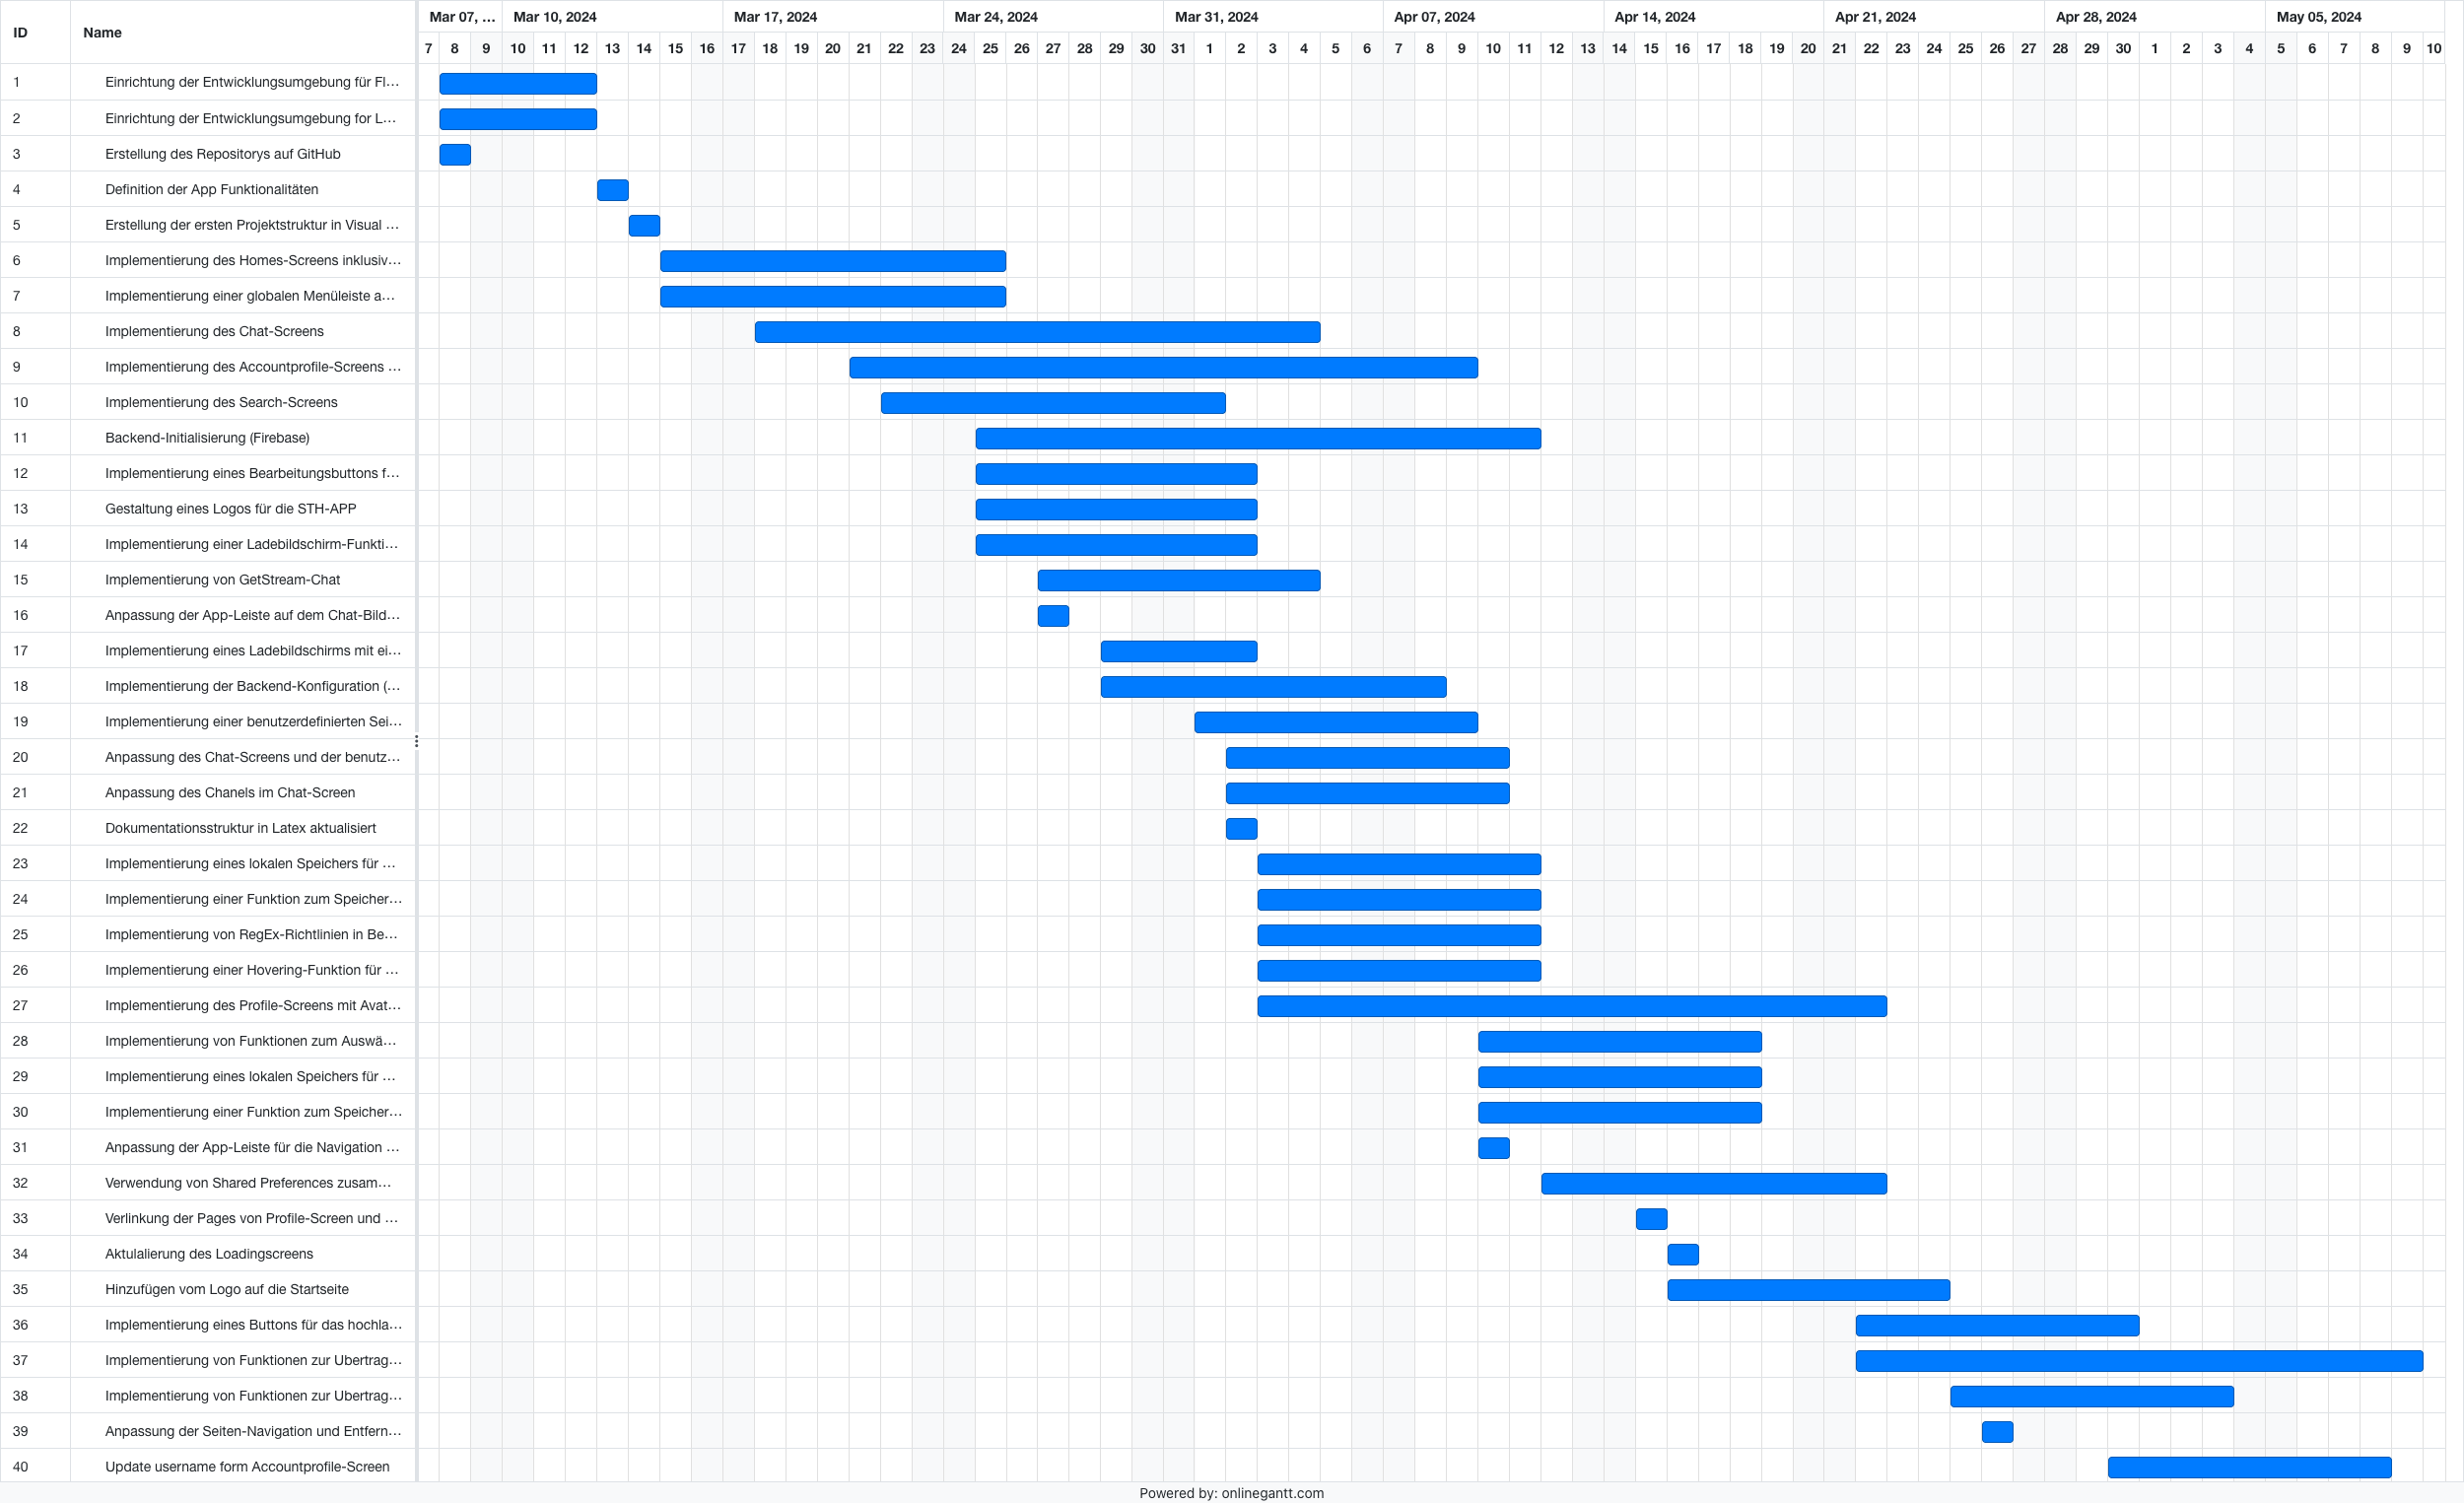
\includegraphics[width=0.9\textwidth]{assets/figures/STH GANTT Diagramm.png}
    \\
    Quelle: Eigene Darstellung über \url{https://www.onlinegantt.com}
\end{figure}
